\question{Ширина спектральной линии излучения. Однородное и неоднородное
уширения линий}

Ширина линии в спектре излучения зависит от множества причин: \\
\begin{enumerate}
    \item  связанные с конечным временем жизни частицы в возбужденном состоянии
        \[
            \begin{array}{c}
                \D E \D\tau \geq \hbar = \frac{h}{2\pi}, \quad
                \D E \geq \cfrac{h}{2\pi\D\tau} \\
                \tau_0 = \D\tau, \quad E = h\nu_0, \quad \D E = h\D\nu_0 \\
                h\D\nu_0 = \cfrac{h}{2\pi\tau_0}, \quad
                \D\nu_0 = \cfrac{1}{2\pi\tau_0}
            \end{array}
        \]
        где \( \D\nu_0 \) -- уширение линии, \( \tau_0 \) -- время жизни
        возбуждённого состояния.
    \item в следствие хаотического движения и столкновений частиц время жизни в
        возбужденном состоянии может сокращаться относительно рассматриваемого
        \( \tau_0 \), что приведёт также к уширению линии
        \[
          \D\nu_\text{ст} = \frac{1}{2\pi\tau_\text{ст}}
            \text{ -- столкновительное уширение}
        \]
        \[
          \tau_\text{ст} = \frac{1}{n\average{\sigma_\text{ст}\cdot v}} =
          \left\{ \begin{array}{c}
            n \text{ -- концентрация} \\
            \sigma_\text{ст} \text{ -- столкновительное сечение} \\
            v \text{ -- скорость}
          \end{array} \right\} = \frac{1}{nk_\text{ст}}
        \]
\end{enumerate}

Уширение линии, связанное с этими причинами называется \emph{однородным
уширением}. Поскольку эти процессы вероятностны, то они описывают распределение
плотности вероятности. Так называемый форм-фактор в данном случае имеет
лоренцев контур:
\begin{gather*}
      \nu_0 = \cfrac{\D E}{h} \\
      q_L(\nu) = \frac{\D\nu_L}{2\pi
        \left[ (\nu-\nu_0)^2 + \left( \frac{\D\nu_L}{2} \right)^2\right]} \\
      \D\nu_L = \D\nu_0 + \D\nu_\text{ст} \\
\end{gather*}
\( \D\nu_L \) -- полная ширина линии на половине высоты.

Уширенными являются все энергетические уровни частицы, за исключением основного
(время жизни основного уровня бесконечно и \( \D\nu = 0 \)).
\begin{enumerate}
    \item[3.] Эффект Доплера.
    В следствие движения частицы относительно приёмника излучения наблюдается
    изменение частоты обусловленное эффектом Доплера.
    \[
      \D\nu_D = \nu_0 \frac{v}{c}\cos\phi
    \]

    Так как излучающие частицы движутся с различными скоростями и в различных
    направлениях, то частотные сдвиги излучаемых ими линий различны. Поэтому даже
    в случае отсутствия столкновений неподвижный спектральный прибор будет
    регистрировать множество естественно уширенных линий, различно смещенных
    относительно частоты \( \nu_0 \). Это так называемое \emph{доплеровское
    уширение}, которое является продуктом деятельности коллектива частиц, такое
    уширение называется \emph{неоднородным}.

    Так как сдвиг определяется скоростью, то форма уширенной линии будет
    определяться распределением частиц по скоростям. При максвелловском
    распределении
    \[
        f(v) = \frac{1}{v_0\sqrt{\pi}}
            \exp\left[-\left(\frac{v}{v_0}\right)^2\right]
    \]
    линия имеет гуссов профиль, описываемый форм-фактором
    \[
        q_G = \frac{c}{v_0\nu_0\sqrt{\pi}}\exp\left[
            -\frac{c^2}{v_0^2}\left(\frac{\nu-\nu_0}{\nu_0}\right)^2
            \right].
    \]
\end{enumerate}
\begin{figure}[h]
  \center
    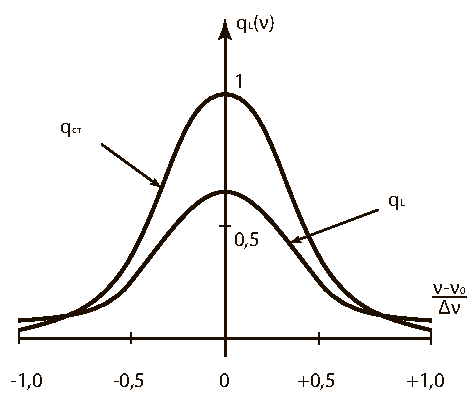
\includegraphics[width=.47\textwidth]{05_01}
\end{figure}
